\documentclass[a4paper, 12pt]{article}%тип документа

%Русский язык
\usepackage[T2A]{fontenc} %кодировка
\usepackage[utf8]{inputenc} %кодировка исходного кода
\usepackage[english,russian]{babel} %локализация и переносы

%абзац
\usepackage{lipsum}
\setlength{\parindent}{5ex}
\setlength{\parskip}{1em}

%Вставка картинок
\usepackage{wrapfig}
\usepackage{graphicx}
\usepackage{placeins}
\graphicspath{{pictures/}}
\DeclareGraphicsExtensions{.pdf,.png,.jpg}

%Графики
\usepackage{multirow}
\usepackage{pgfplots}
\pgfplotsset{compat=1.9}

%Математика
\usepackage{amsmath, amsfonts, amssymb, amsthm, mathtools}

\begin{document}

\section{\textbf{model4}}

\subsection*{Полосовой RC-фильтр}

\begin{enumerate}

\item

Объяснение:

На низких частотах емкостной импеданс велик и шум на выходе это шум $e_2$ одного резистора R. На высоких частотах малый импеданс емкостей эффективно закорачивает выход, делая выходной шум малым. Коэффициент передачи имеет максимум на частоте $f_0$. Спад коэффициента передачи на низких частотах при постоянстве уровня шума на выходе обеспечивает резкий рост коэффициента шума.

Формула коэффициента шума $K = 20 lg \left( \frac{e_n(f)}{\sqrt{4 k T R}} \right)$

\FloatBarrier
\begin{figure}
    \centering
    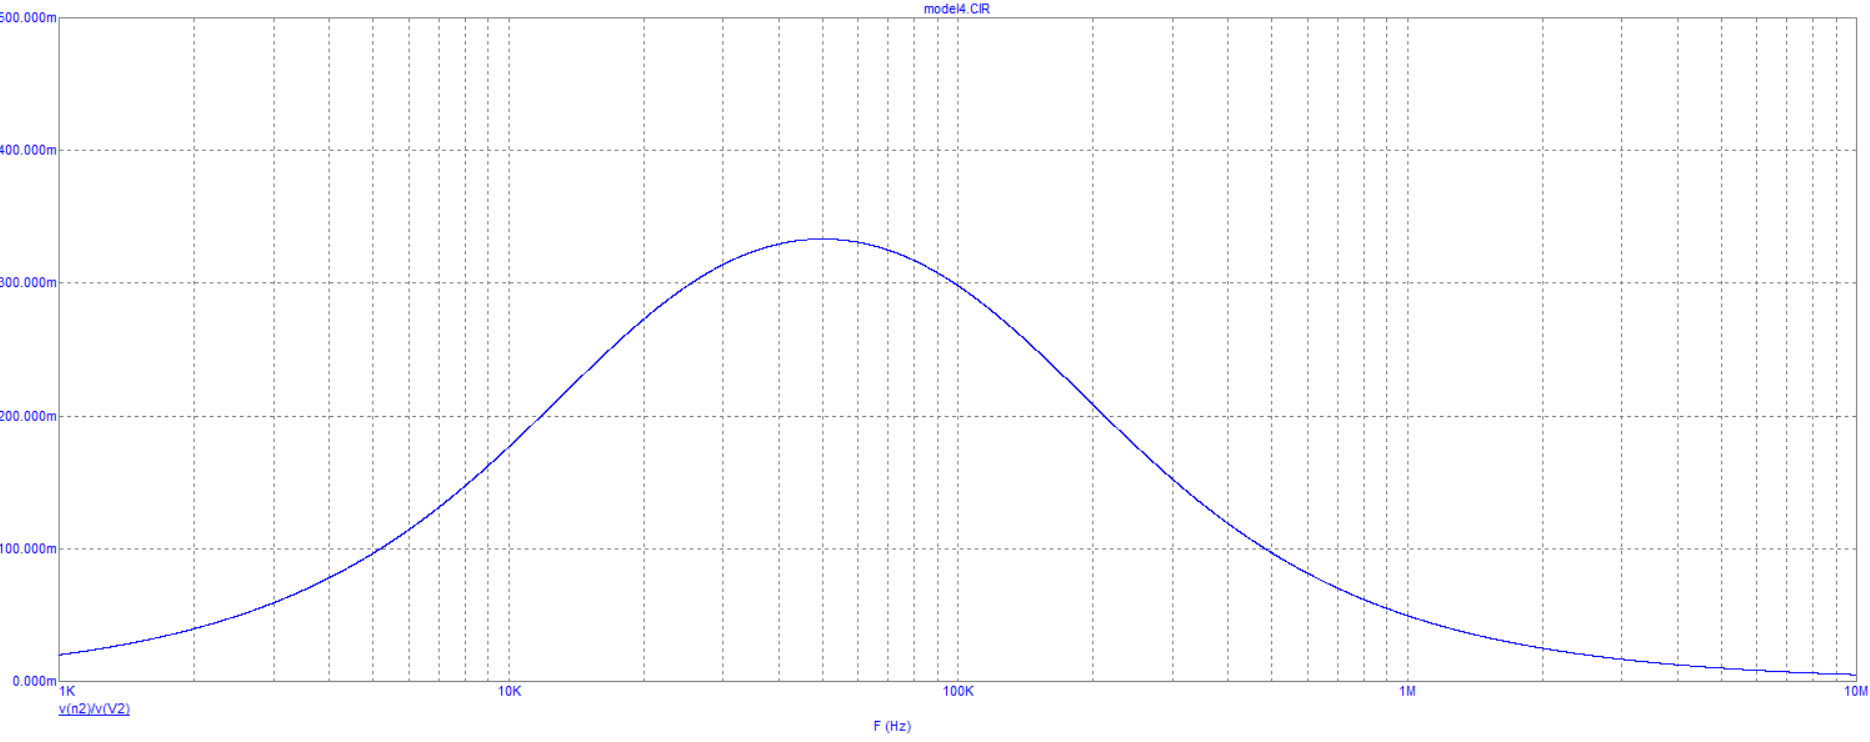
\includegraphics[scale=0.3]{images/mod4_2_1.png}
    \caption{$f_0 = 50k, \Delta f = 152k, K = 0.33$, с теорией сходится}
    \label{fig:m421}
\end{figure}

\begin{figure}
    \centering
    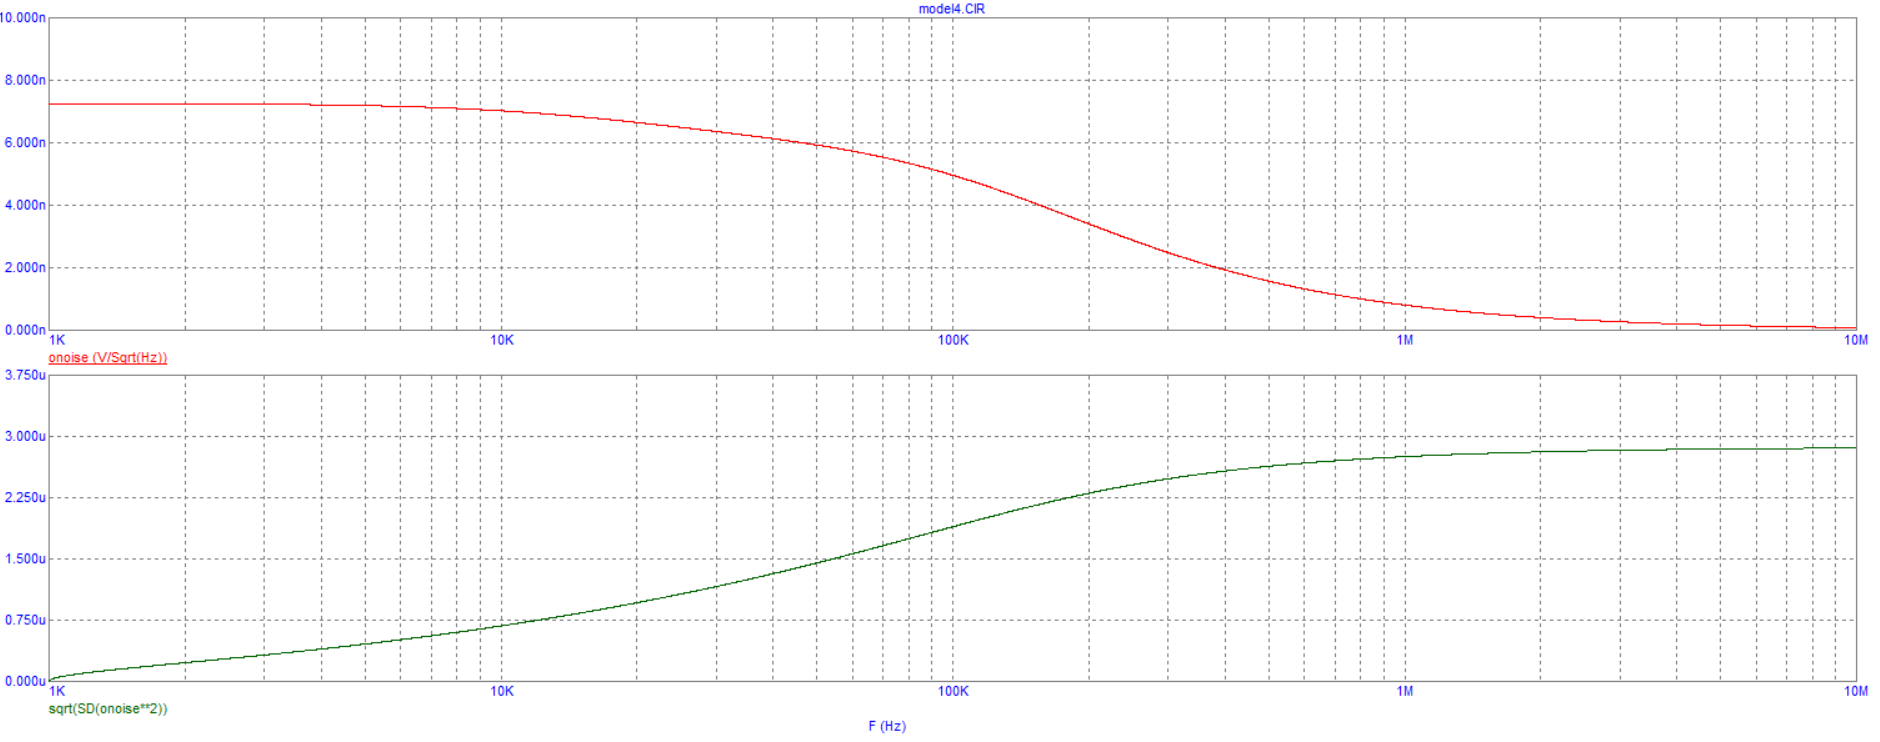
\includegraphics[scale=0.3]{images/mod4_2_2_1.png}
    \caption{$n(f_0) = 5.88n, n(10 f_0) = 1.56n, \sigma = 2.86\mu$, оба резистора шумящие}
    \label{fig:m4221}
\end{figure}

\begin{figure}
    \centering
    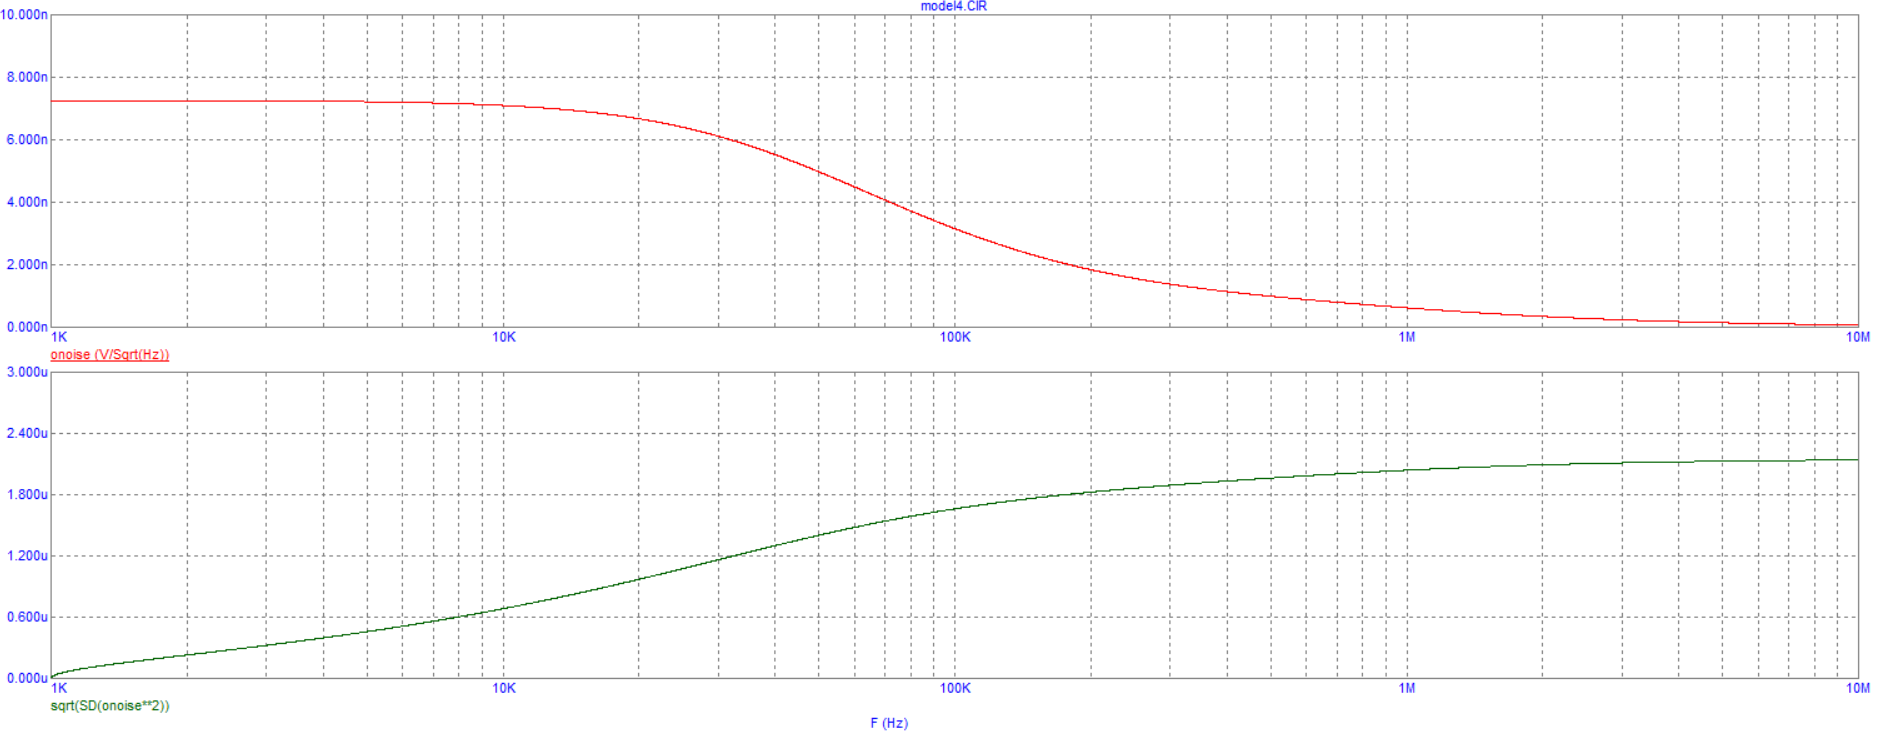
\includegraphics[scale=0.3]{images/mod4_2_2_2.png}
    \caption{$n(f_0) = 4.96n, n(10 f_0) = 960p, \sigma = 2.15\mu, R_{s_2}$ не шумящий}
    \label{fig:m4222}
\end{figure}

\begin{figure}
    \centering
    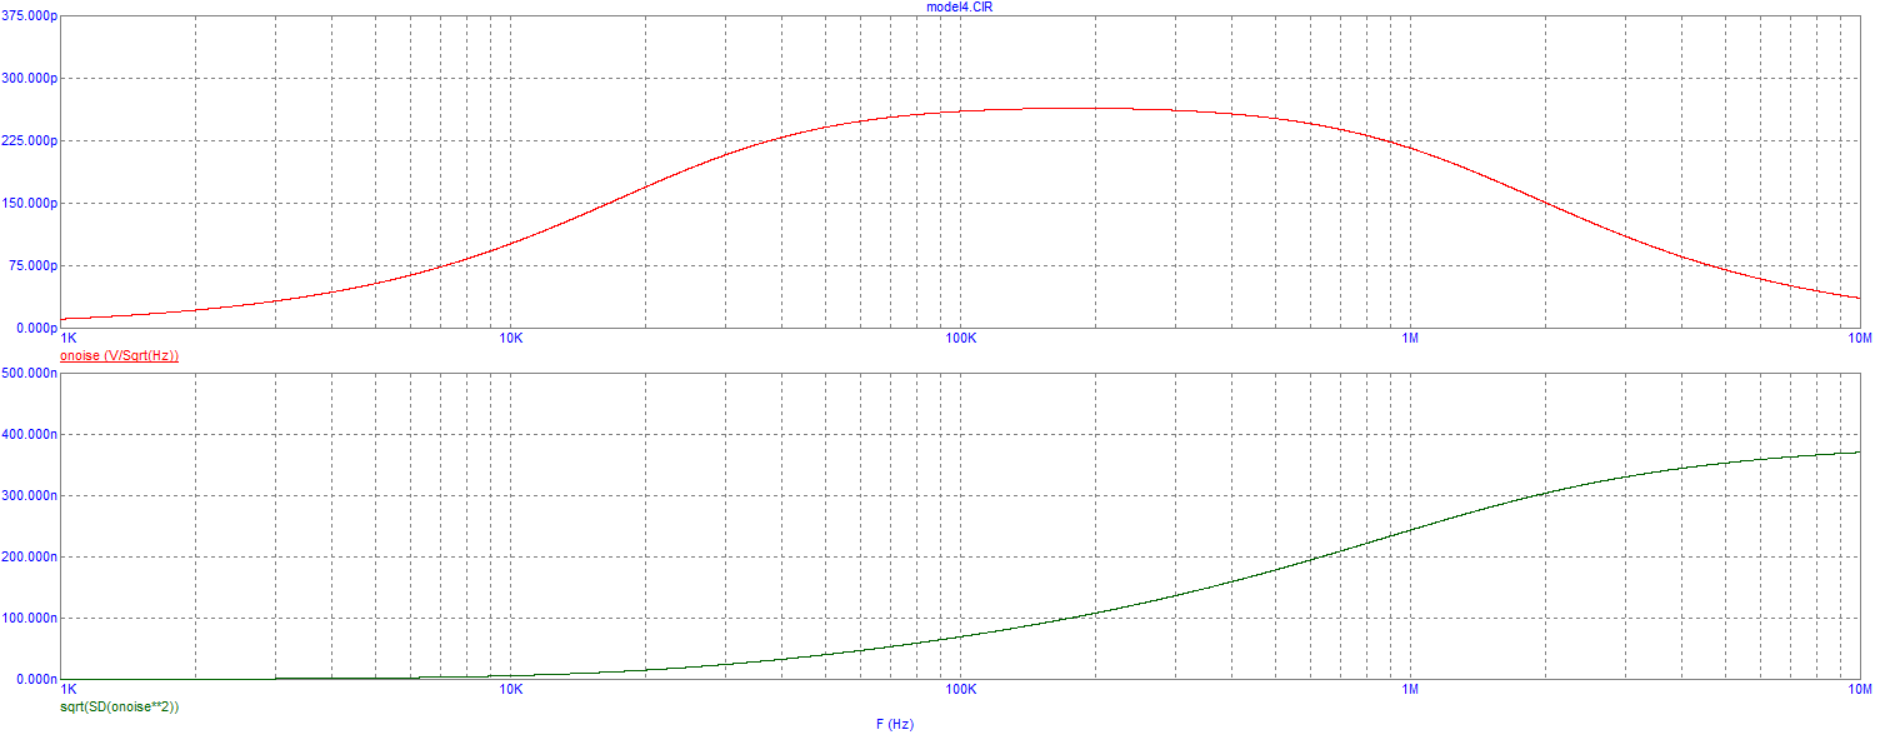
\includegraphics[scale=0.3]{images/mod4_2_2_3.png}
    \caption{$n(f_0) = 240p, n(10 f_0) = 250p, \sigma = 370n,  R_2$ нешумящий}
    \label{fig:m4223}
\end{figure}

\begin{figure}
    \centering
    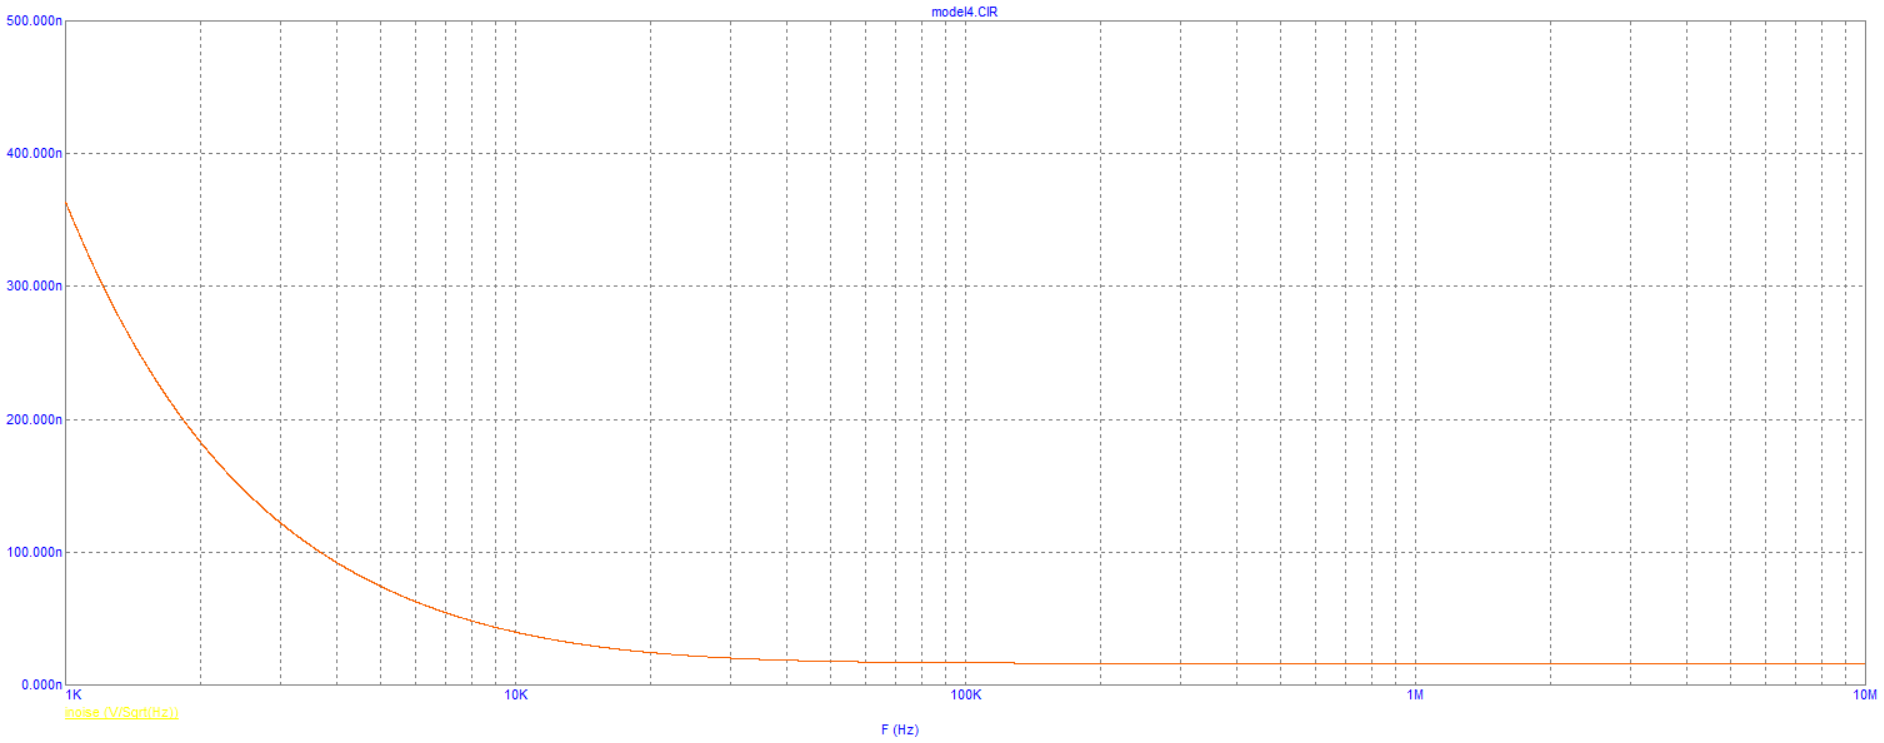
\includegraphics[scale=0.3]{images/mod4_2_3.png}
    \caption{$e(f_0) = 17.7n, e(f_0/10) = 73.45n, e(f_0/100) = 728.6n => K(f_0) = 7.9, K(f_0/10) = 20.4, K(f_0/100) = 41$}
    \label{fig:m423}
\end{figure}
\FloatBarrier


\end{enumerate}

\subsection*{Полосовой LC-фильтр нижних частот}

На низких частотах индуктивный импеданс мал, а емкостный велик. При этом шум на выходе создается параллельным соединением r||R и отличен от нуля. С учетом малости коэффициента передачи это приводит к высокому уровню коэффициента шума. На высоких частотах большой индуктивный импеданс эффективно отключает резистор r. Получается обычная интегрирующая RC-цепь с нулевым коэффициентом шума. Таким образом, в фильтре на параллельном контуре с омическим сопротивлением индуктивности r обнаруживается рост коэффициента шума на частотах ниже резонанса.

Формула коэффициента шума $K = 20 lg \left( \frac{e_n(f)}{\sqrt{4 k T R}} \right)$

\begin{enumerate}

\item

\FloatBarrier
\begin{figure}[h!]
    \centering
    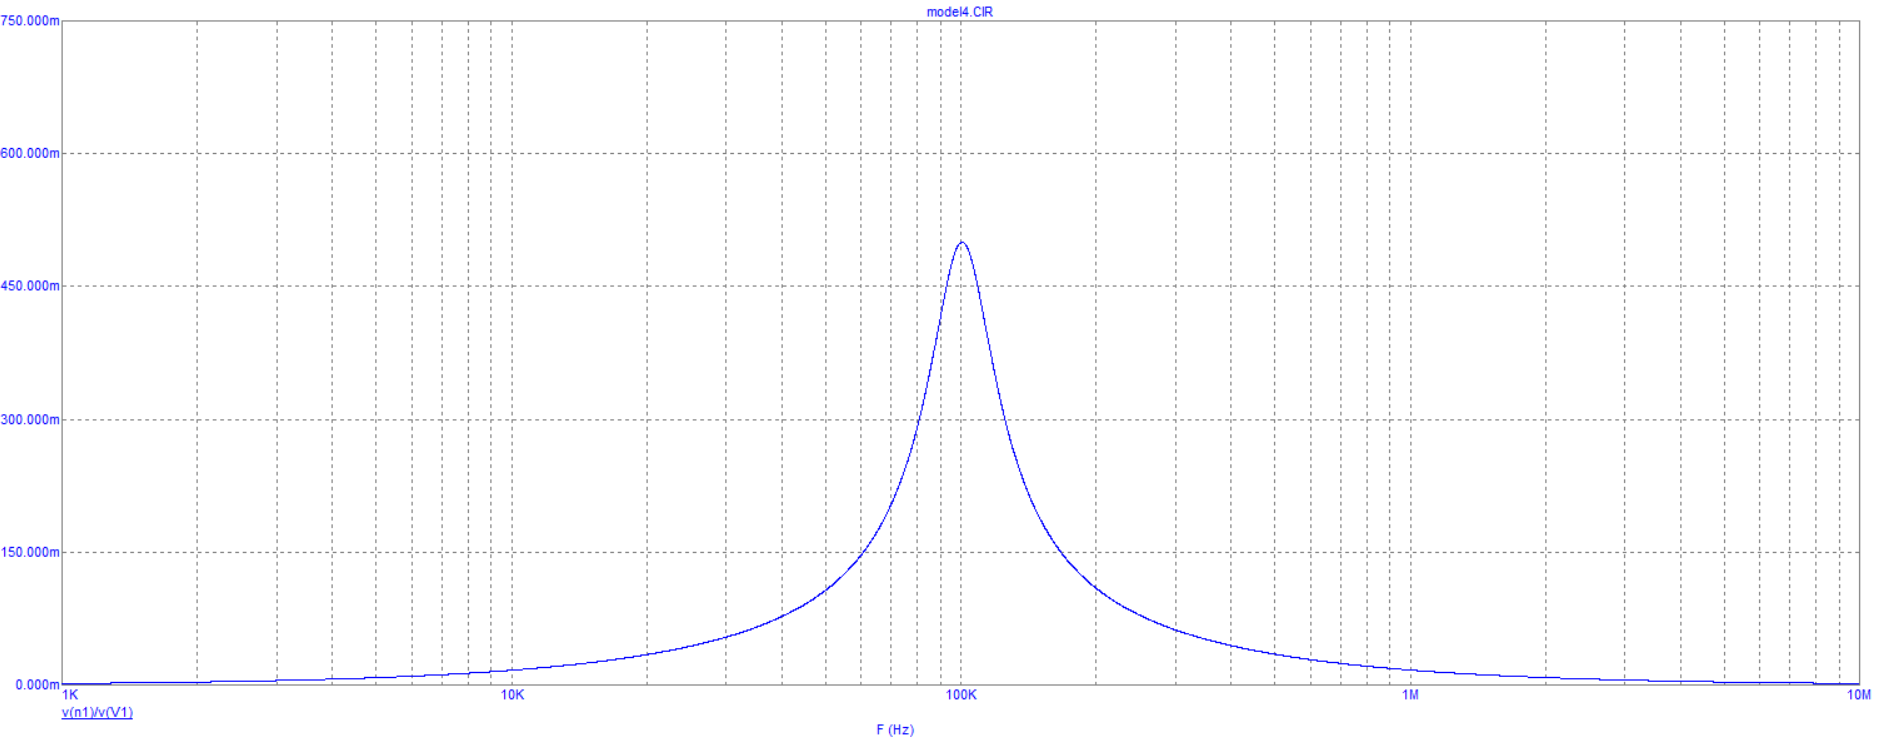
\includegraphics[scale=0.3]{images/mod4_3_1.png}
    \caption{$f_0 = 102k, \Delta f = 36k, K(f_0) = 0.5, K(0) = 0.02$, с теорией сходится}
    \label{fig:m431}
\end{figure}

\begin{figure}[h!]
    \centering
    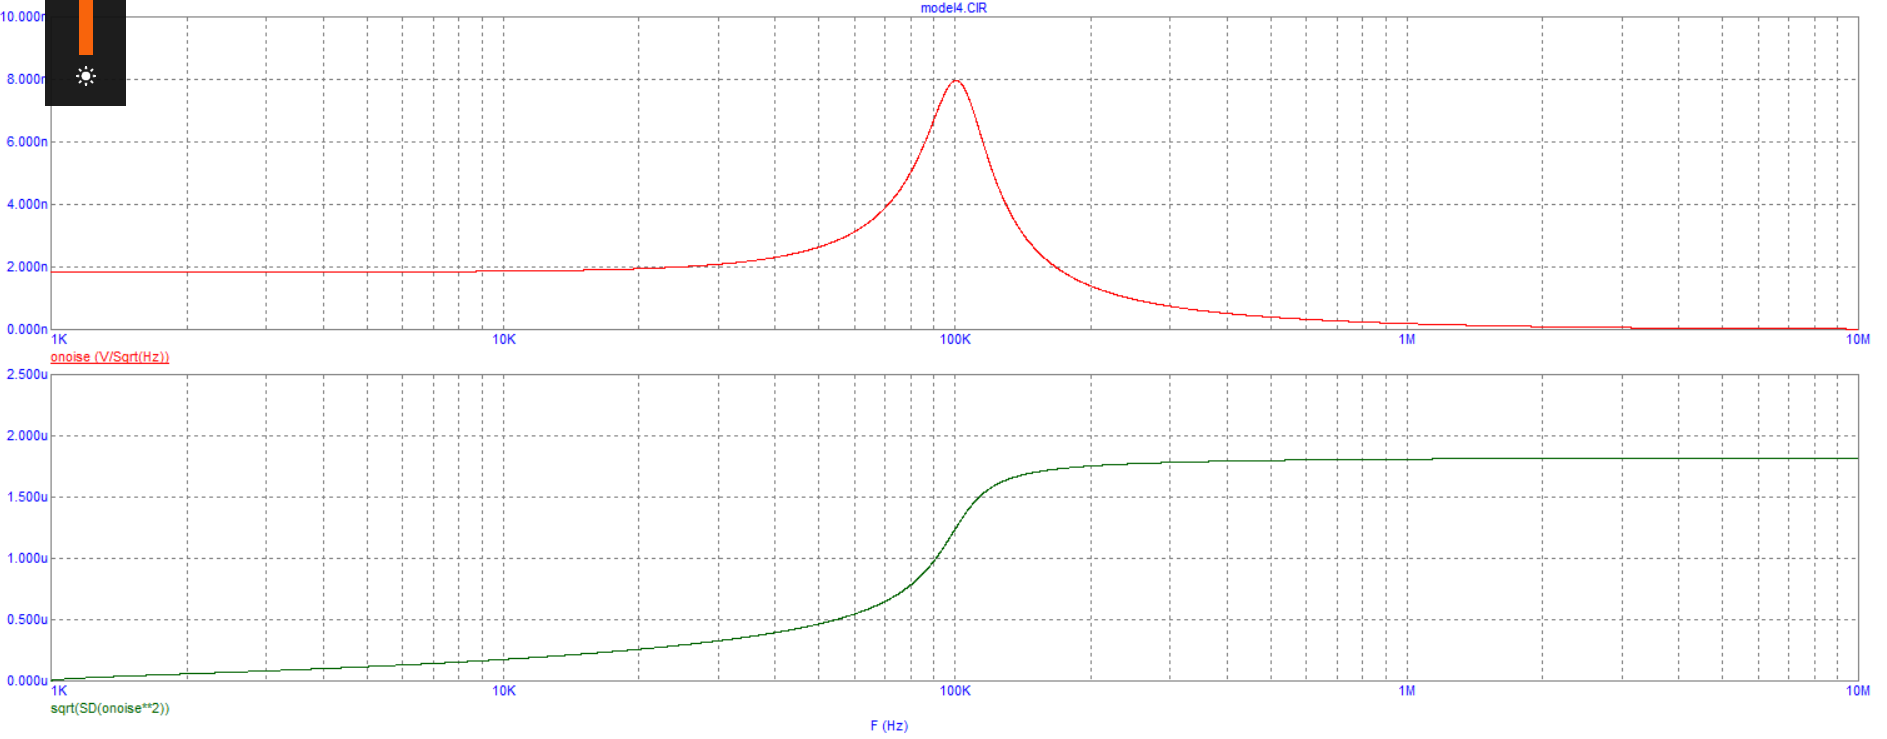
\includegraphics[scale=0.3]{images/mod4_3_2_1.png}
    \caption{$n(f_0) = 7.9n, n(f_0/100) = 1.8n, \sigma = 1.8\mu$, оба шумящие}
    \label{fig:m4321}
\end{figure}

\begin{figure}[h!]
    \centering
    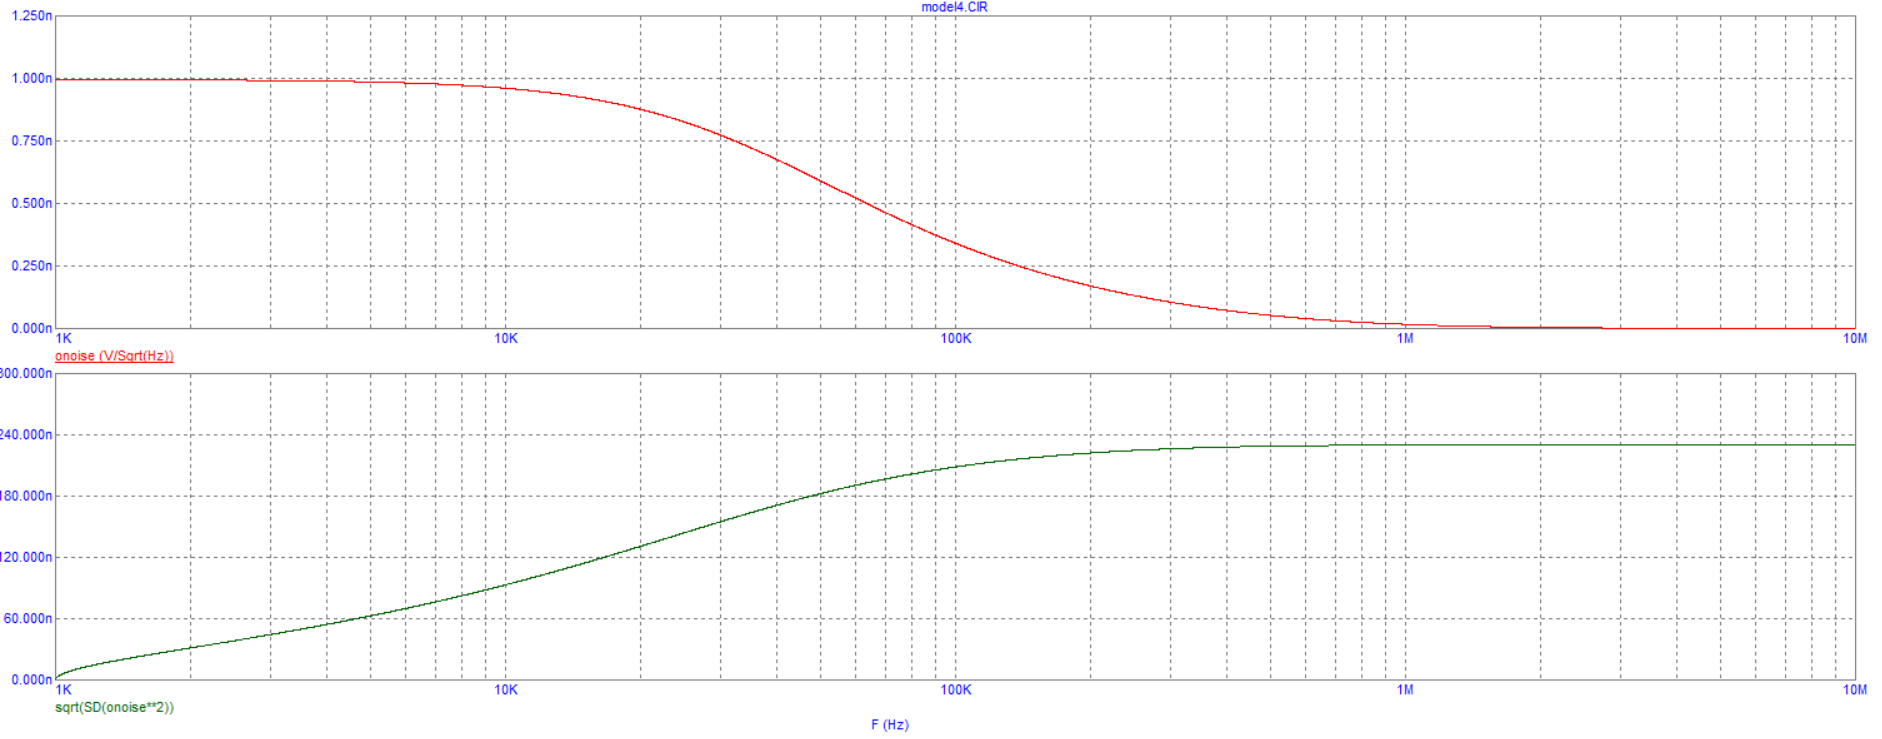
\includegraphics[scale=0.3]{images/mod4_3_2_2.png}
    \caption{$n(f_0) = 355p, n(f_0/100) = 1.0n, \sigma = 228.9n, R_3$ шумящий}
    \label{fig:m4322}
\end{figure}

\begin{figure}[h!]
    \centering
    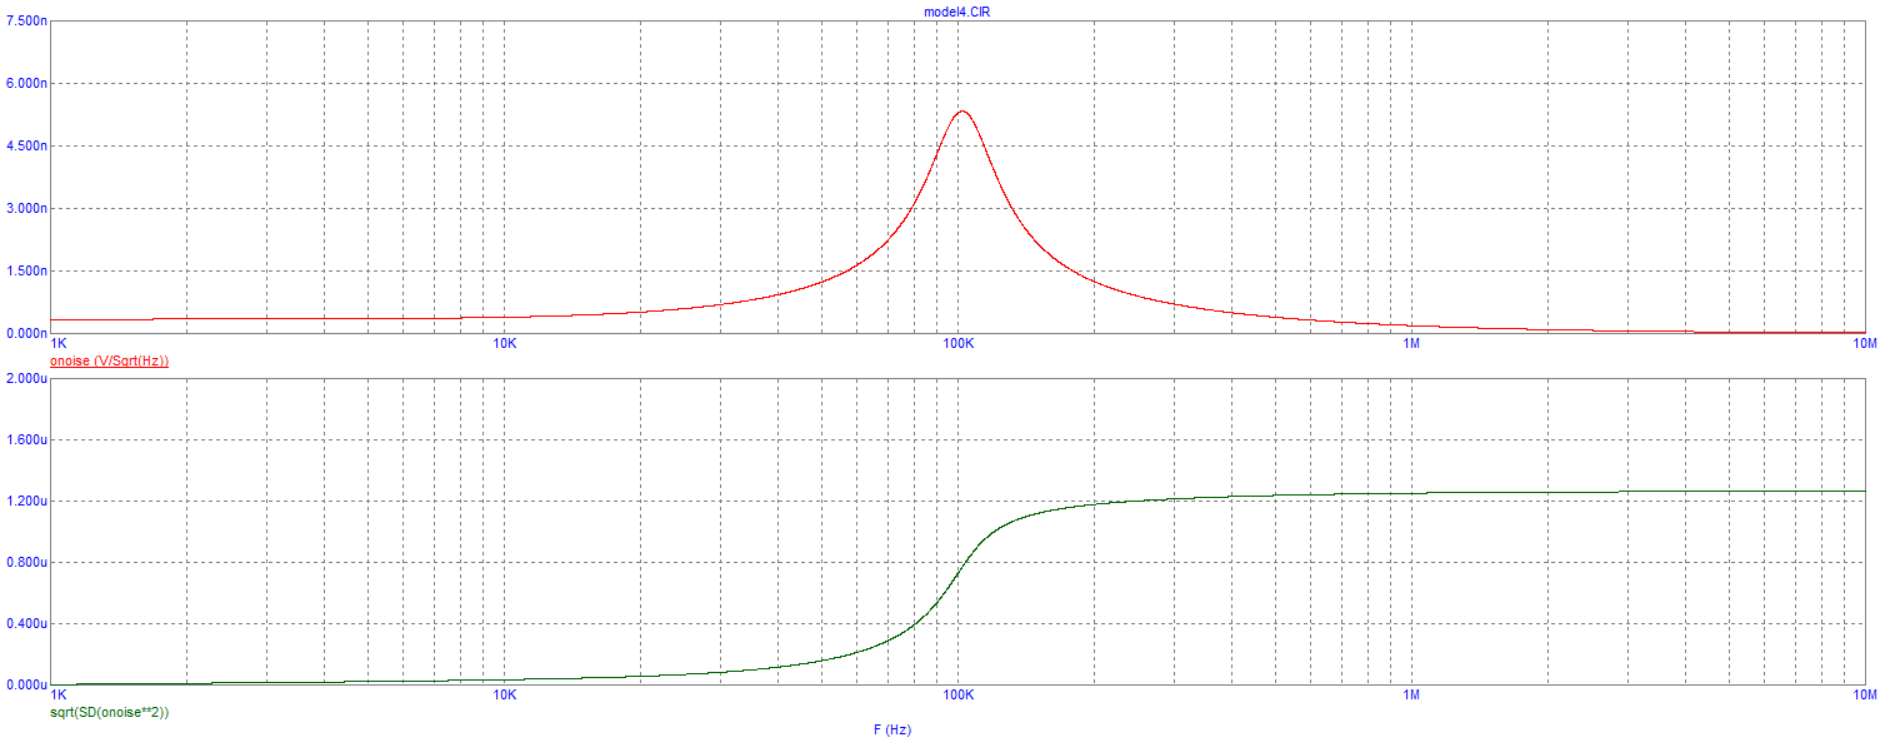
\includegraphics[scale=0.3]{images/mod4_3_2_3.png}
    \caption{$n(f_0) = 1.8n, n(f_0/100) = 11.2n, \sigma = 1.7\mu, R_{s3}$ шумящий}
    \label{fig:m4322}
\end{figure}

\begin{figure}[h!]
    \centering
    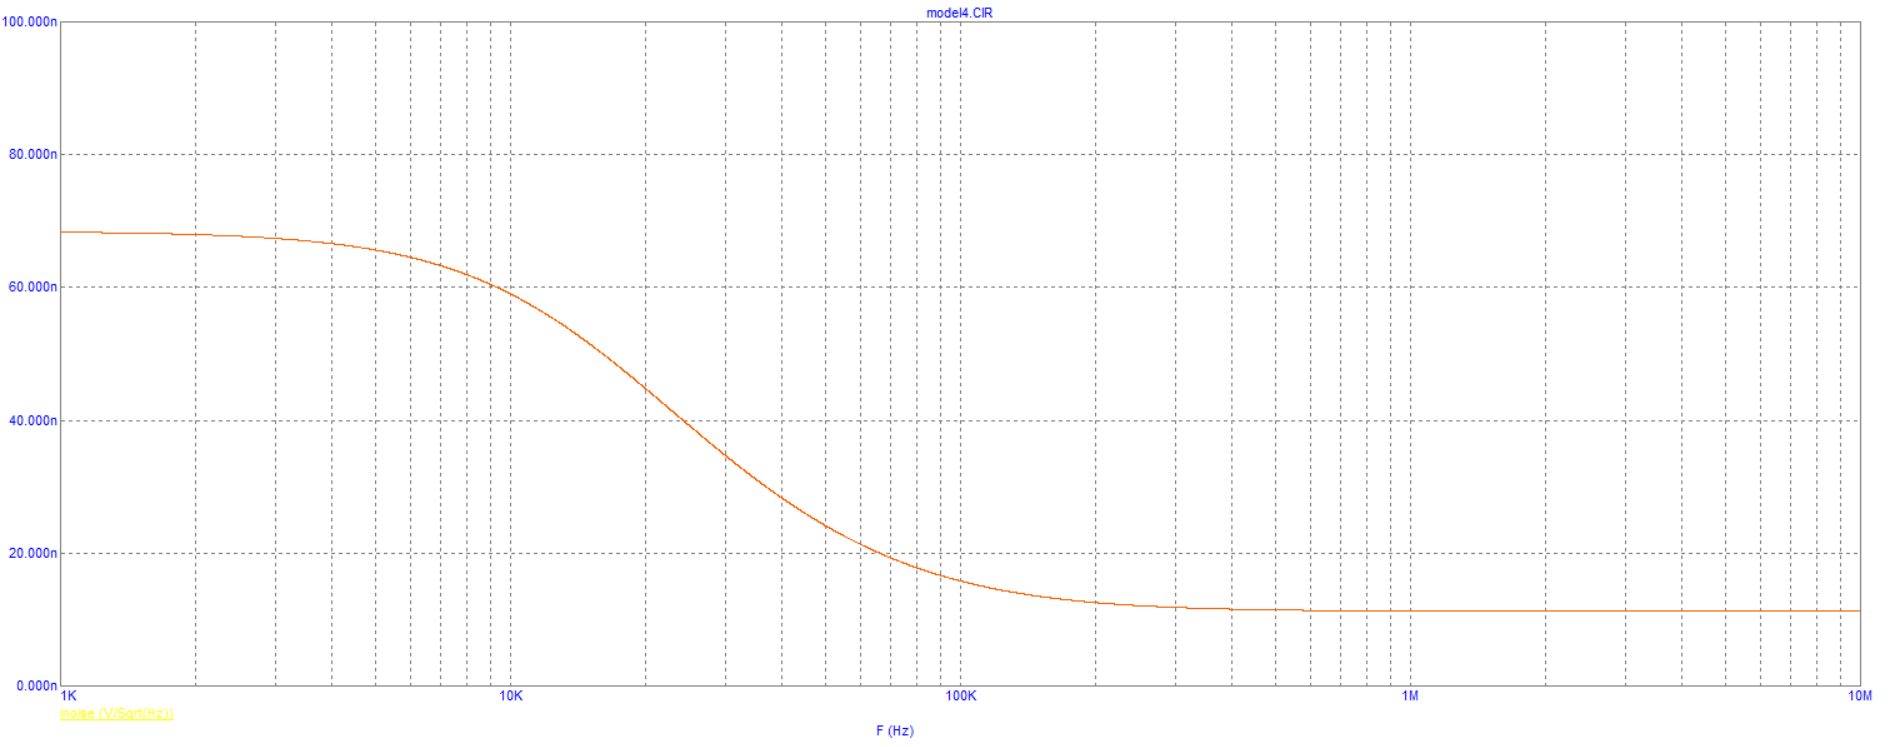
\includegraphics[scale=0.3]{images/mod4_3_3.png}
    \caption{$e(f_0) = 15.4n, e(f_0/100) = 68.3n, e(10 f_0) = 10.9n => K(f_0) = 31.5, K(f_0/100) = 18.9, K(10 f_0) = 15.8$}
    \label{fig:m433}
\end{figure}
\FloatBarrier


\end{enumerate}

\section{\textbf{model5}}

\begin{enumerate}

\item

\FloatBarrier
$I_c = 1 \text{ мА}, r_b = 100$ Ом

Такой ток соответствует $I_1 = 13.5$ мкА.

\end{enumerate}

\subsection*{Измерение шумового коллекторного тока}

\begin{enumerate}

\FloatBarrier
\item
\FloatBarrier
\begin{figure}
    \centering
    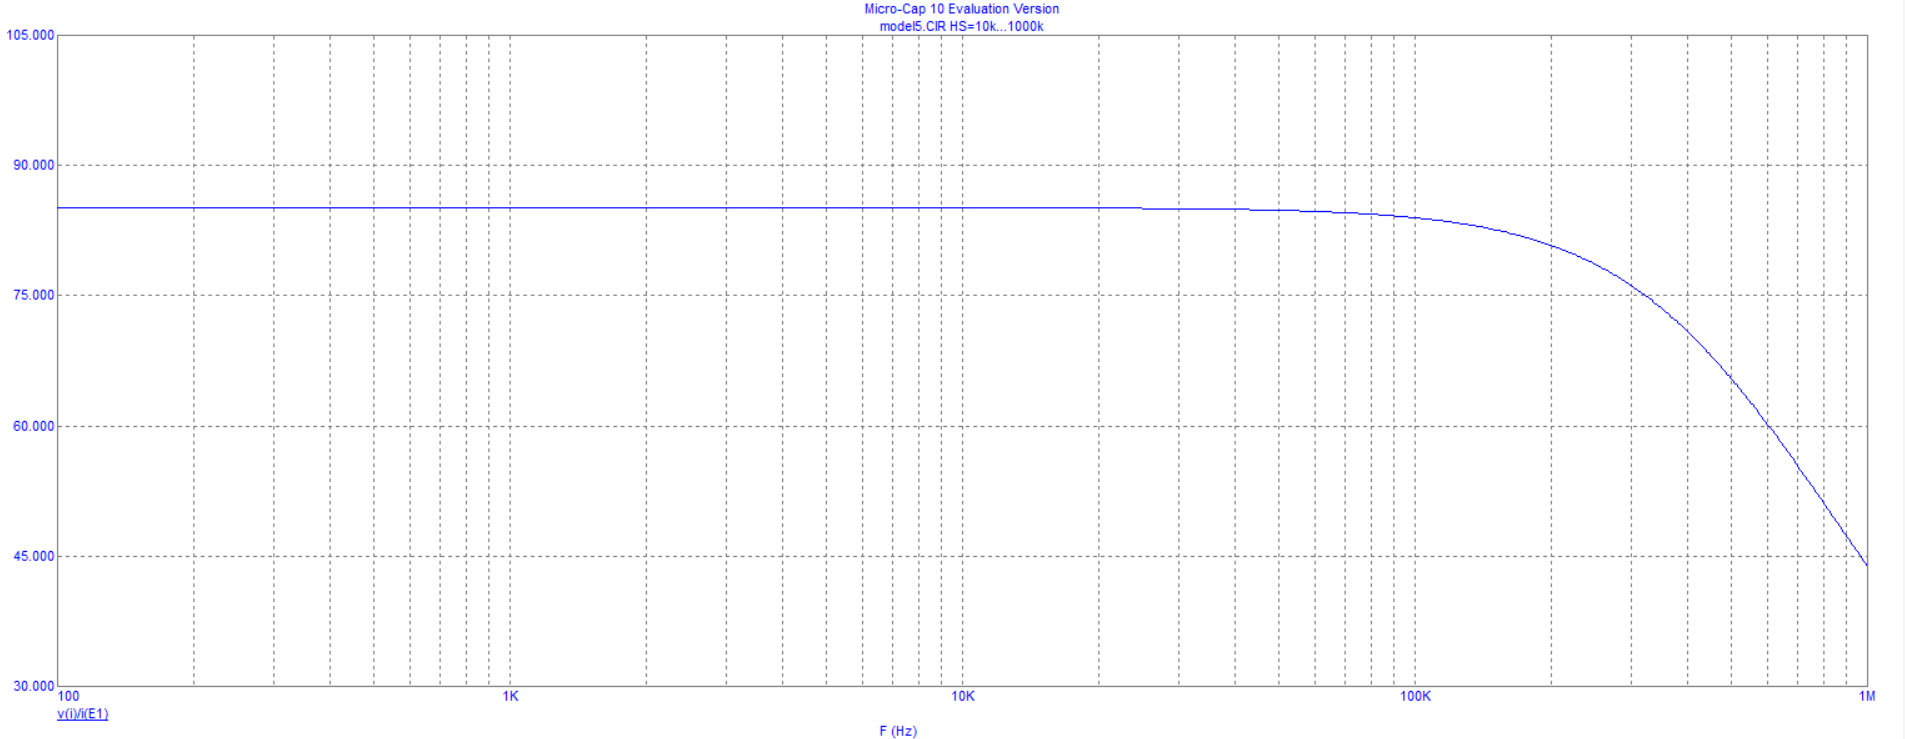
\includegraphics[scale=0.225]{images/mod5_1_1.png}
    \caption{$h_{21}$ = 85.1}
    \label{fig:m511}
\end{figure}
\FloatBarrier
\item
\FloatBarrier
\begin{figure}[h!]
    \centering
    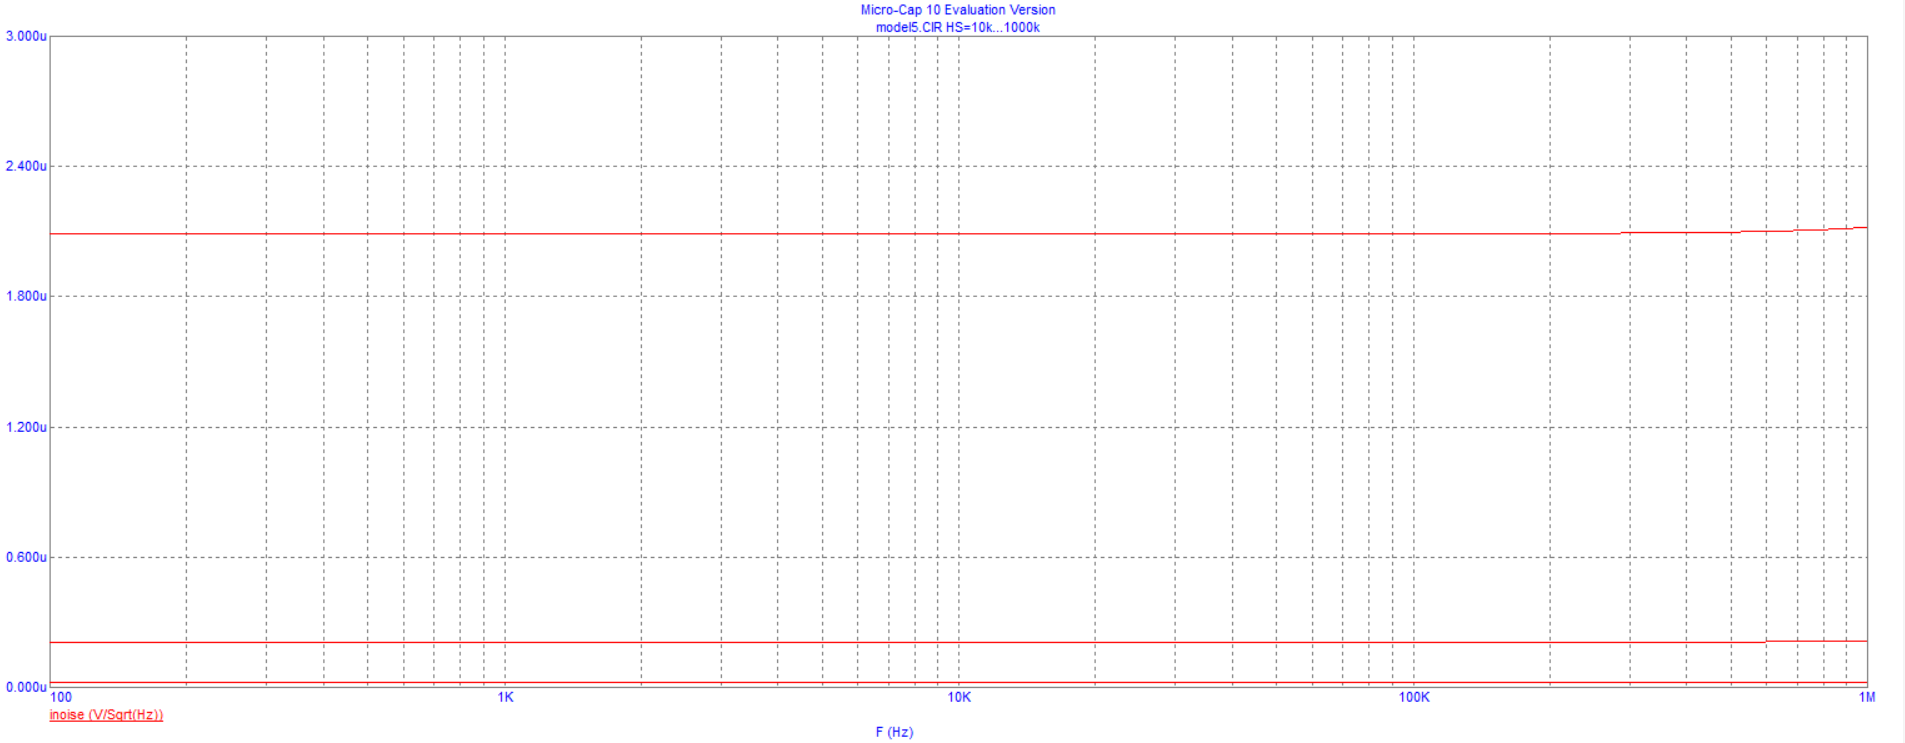
\includegraphics[scale=0.225]{images/mod5_1_2_1.png}
    \caption{Варьирование $H_s = [10, 1000k|Log10]$}
    \label{fig:m5121}
\end{figure}

\begin{figure}[h!]
    \centering
    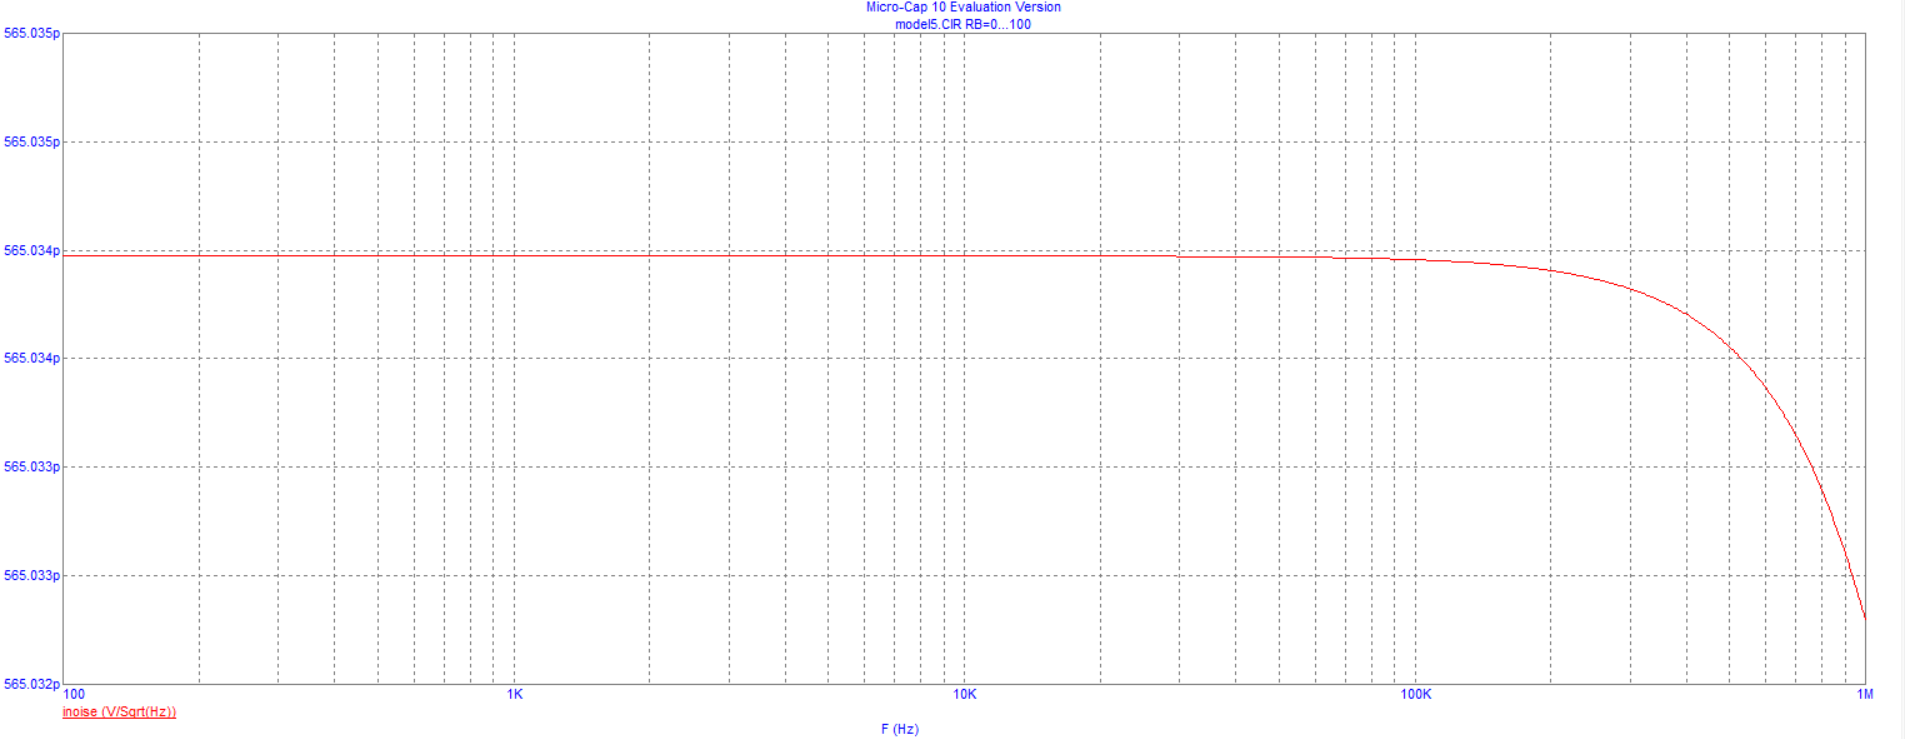
\includegraphics[scale=0.225]{images/mod5_1_2_2.png}
    \caption{Варьирование $RB = [0, 100|25]$}
    \label{fig:m5122}
\end{figure}
\FloatBarrier
\item
\FloatBarrier
\begin{figure}
    \centering
    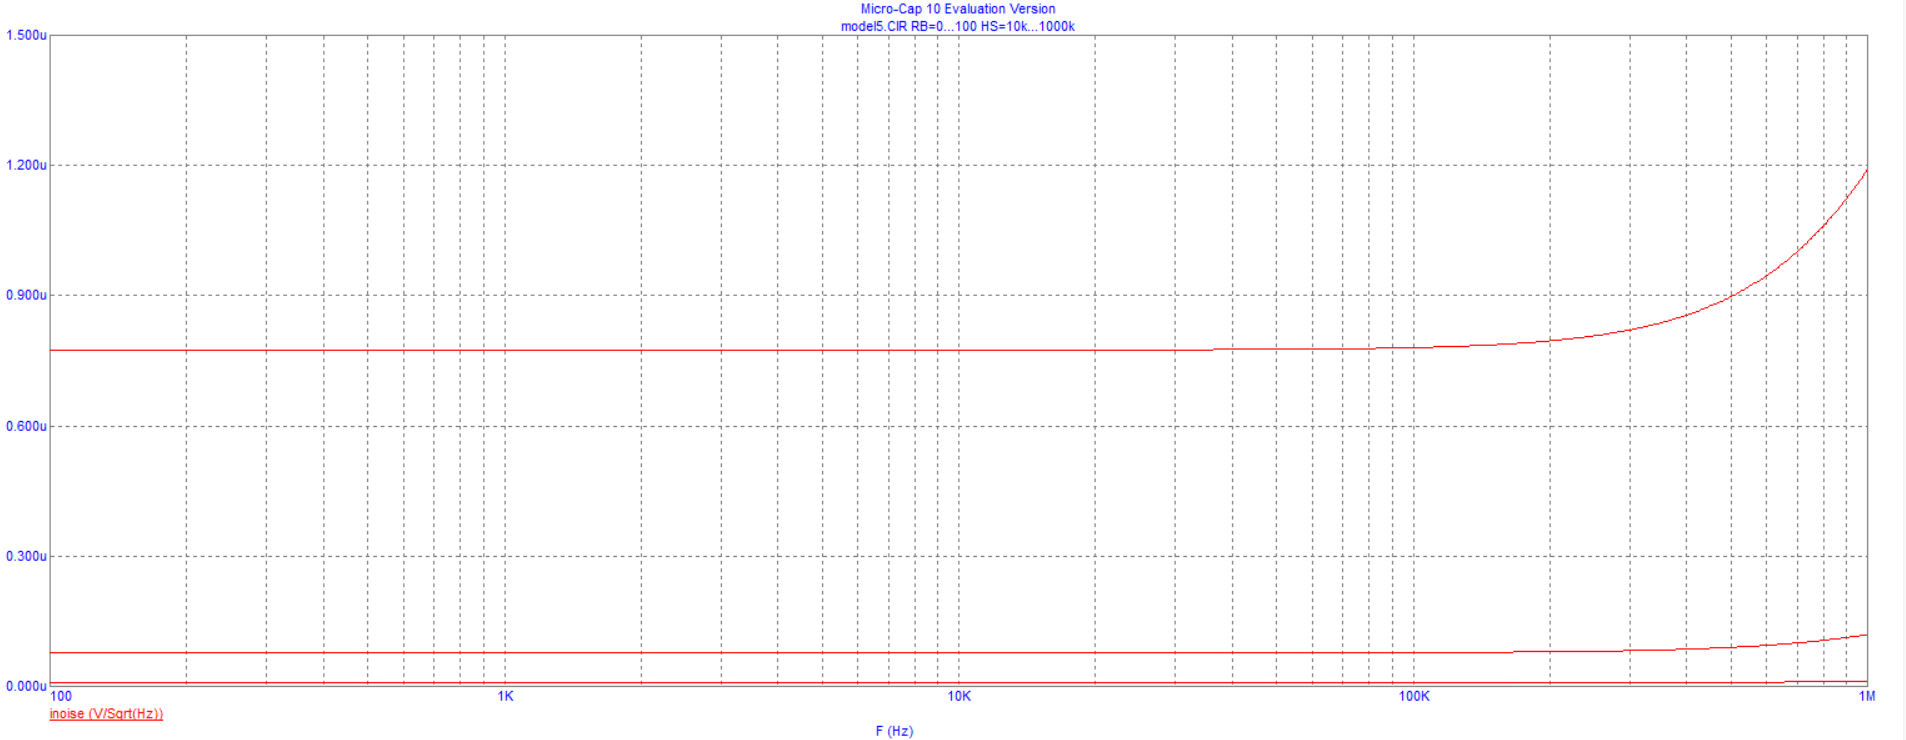
\includegraphics[scale=0.225]{images/mod5_1_3_1.png}
    \caption{Варьирование $H_s = [10, 1000|Log10]$ для $I_c = 0.1m, I_1 = 1.83\mu$}
    \label{fig:m5131}
\end{figure}

\begin{figure}[h!]
    \centering
    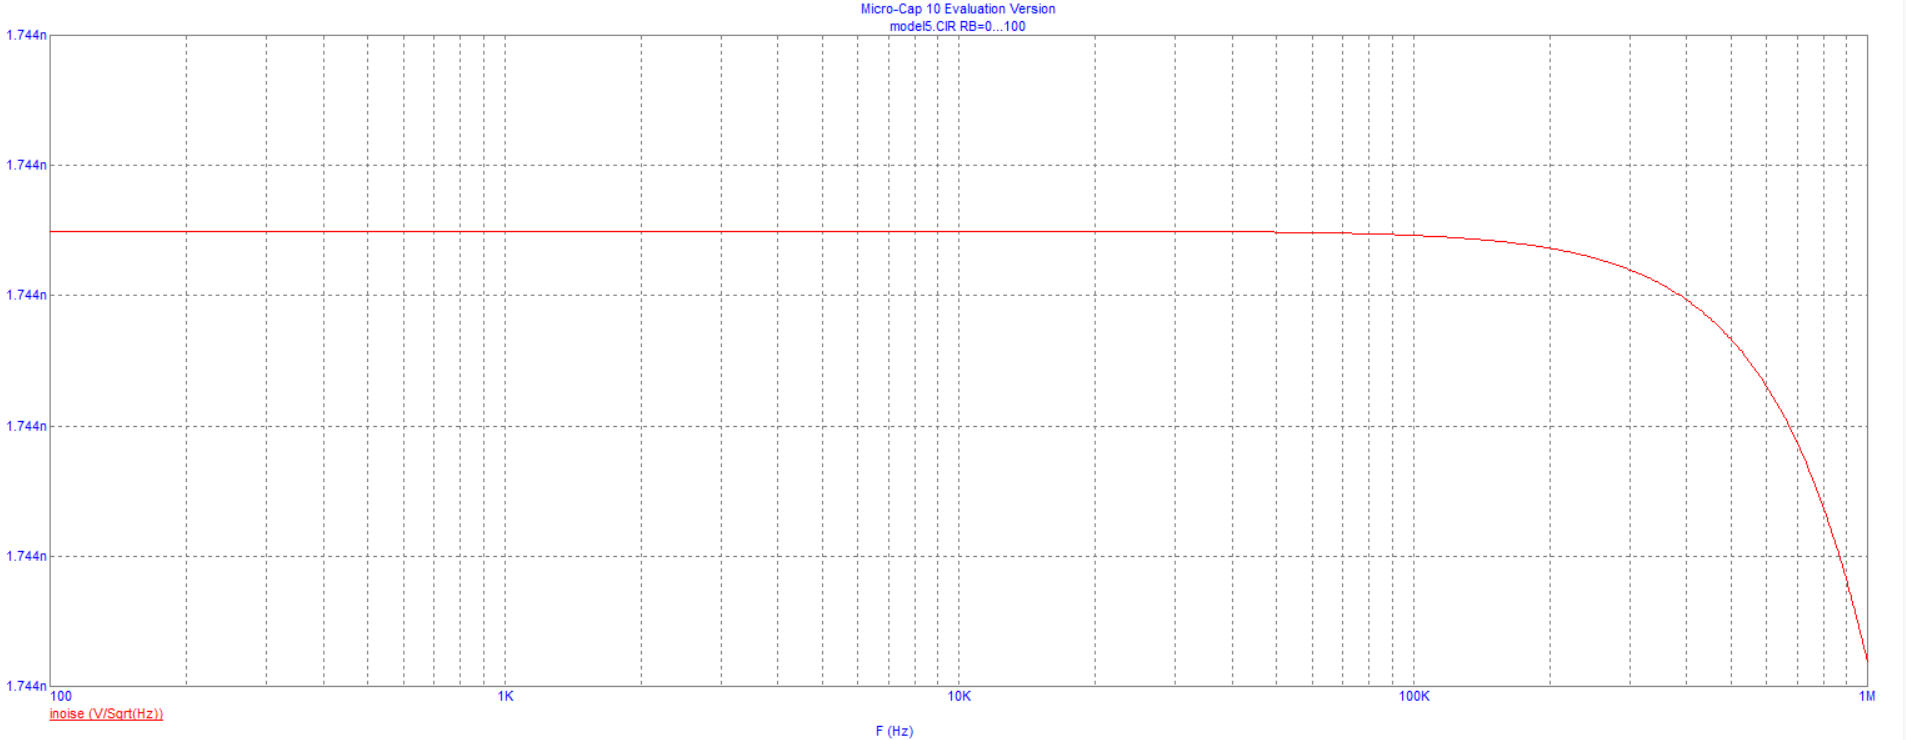
\includegraphics[scale=0.225]{images/mod5_1_3_2.png}
    \caption{Варьирование $RB = [0, 100|25]$ для $I_c = 0.1m, I_1 = 1.83\mu$}
    \label{fig:m5132}
\end{figure}
\FloatBarrier

Варьирование $H_s$ ожидаемо дает различные значения тока на выходе, причем при больших сопротивлениях ток больше. От сопротивления ток на коллекторе зависит линейно, т.е. увеличивается в 10 раз при шаге варьирования.

При уменьшении подаваемого тока нелинейно падает ток на коллекторе.

Варьируя объемное сопротивление базы при нулевом сопротивлении $H_s$, подаваемый ток с $H_s$ равен нулю, а вклад остается только у теплового шума объемного сопротивления базы, что и повышает ток при увеличении тока пропорционально корню из его значения $\left( I_c \cdot r \right)$.

\end{enumerate}

\subsection*{Измерение коэффициента шума}

\begin{enumerate}
\item

\FloatBarrier
$R_s$ = 40k.

\begin{figure}[h!]
    \centering
    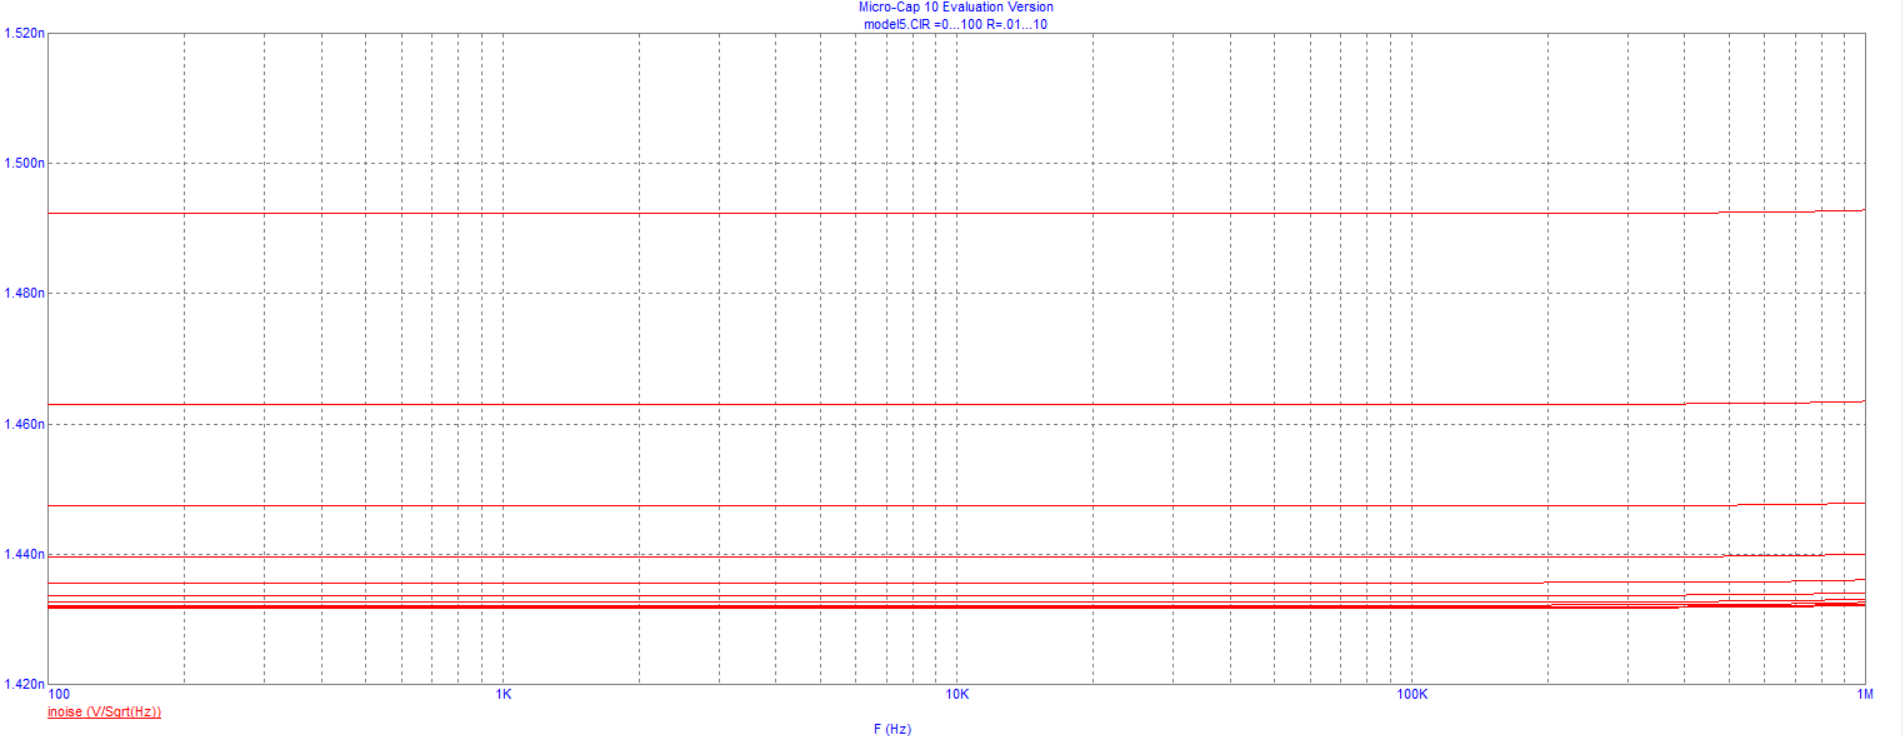
\includegraphics[scale=0.3]{images/2023-11-23_17-00-00.png}
    \caption{Шумовой ток, варьирование $R$}
    \label{fig:m612}
\end{figure}

При низком сопротивлении R коэффициент шума падает, и в пределе  i = $1.42$ нА. Шумовая температура составит $T = 300$ К, а усилителя $R_n = 5$ кОм. На выходе $\sigma \approx 200$ нА.


\end{enumerate}

\section{\textbf{model6}}

\begin{enumerate}

\item

$U_p = 1.1$ В, $R_g = 25$ Ом, $I_d = 1m?$
\FloatBarrier


\end{enumerate}

\subsection*{Исследование шумового тока}

\begin{enumerate}

\item

\FloatBarrier
\begin{figure}[h!]
    \centering
    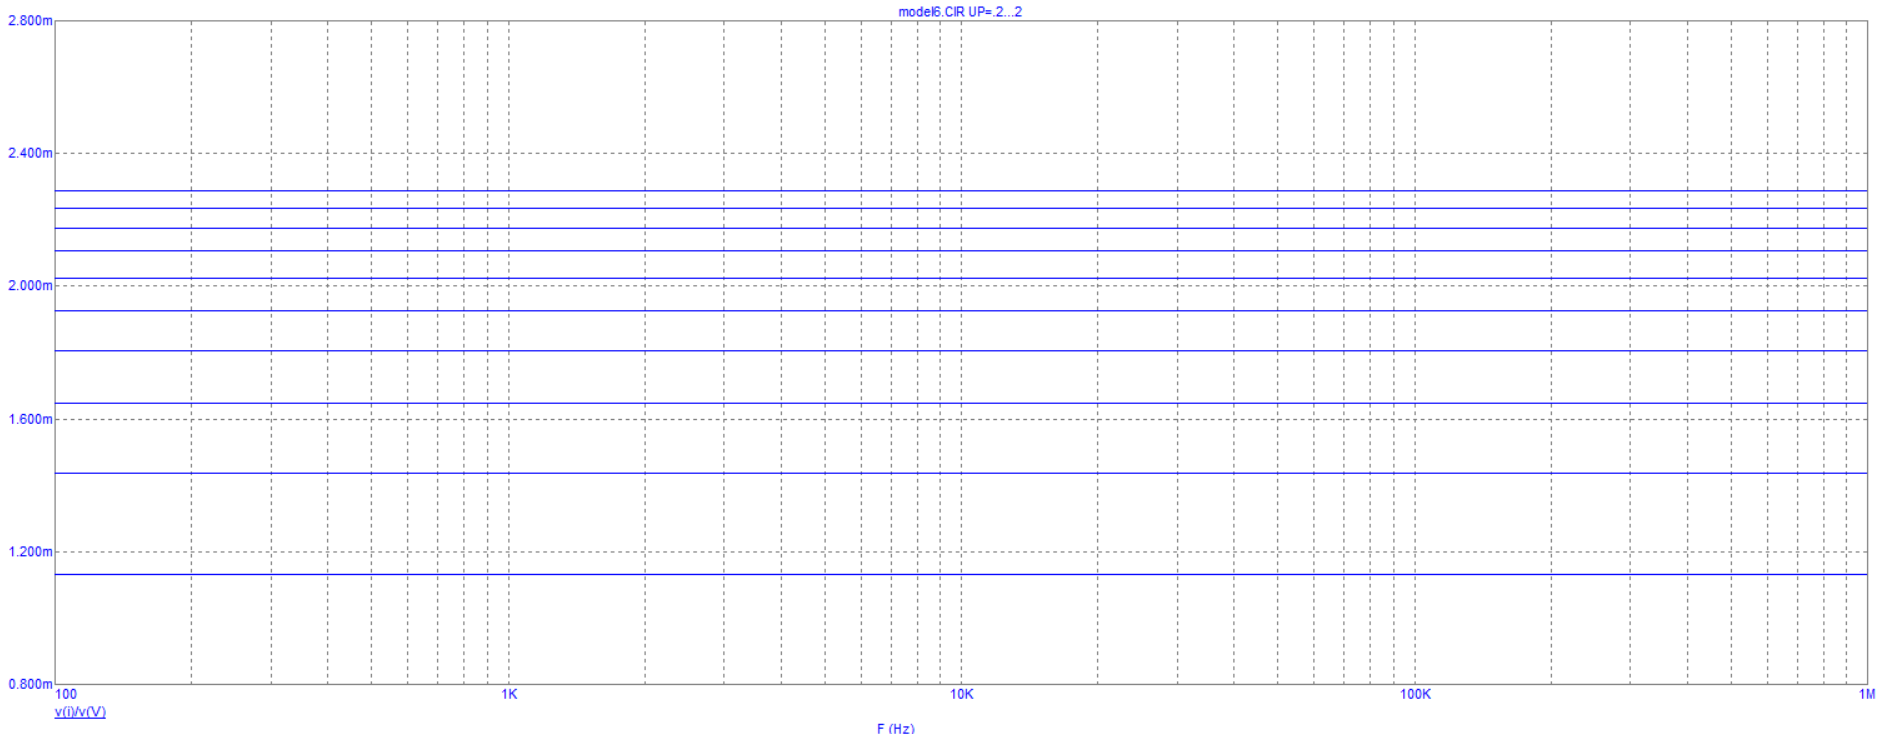
\includegraphics[scale=0.3]{images/mod6_1_1.png}
    \caption{Крутизна транзистора}
    \label{fig:m611}
\end{figure}

\begin{center}
\begin{table}[h!]
    \centering
    \begin{tabular}{|c|c|c|c|c|c|c|c|c|c|c|}
    \hline
        $U_p$ & 2 & 1.8 & 1.6 & 1.4 & 1.2 & 1.0 & 0.8 & 0.6 & 0.4 & 0.2\\ \hline
        $S$ & 1.13 & 1.44 & 1.65 & 1.80 & 1.92 & 2.02 & 2.11 & 2.18 & 2.24 & 2.29 \\ \hline
    \end{tabular}
    \caption{Для $U_p = 1.1 V \, \frac{1}{S} \approx 0.5$}
    \label{tab:my_label}
\end{table}
\end{center}

\begin{figure}[h!]
    \centering
    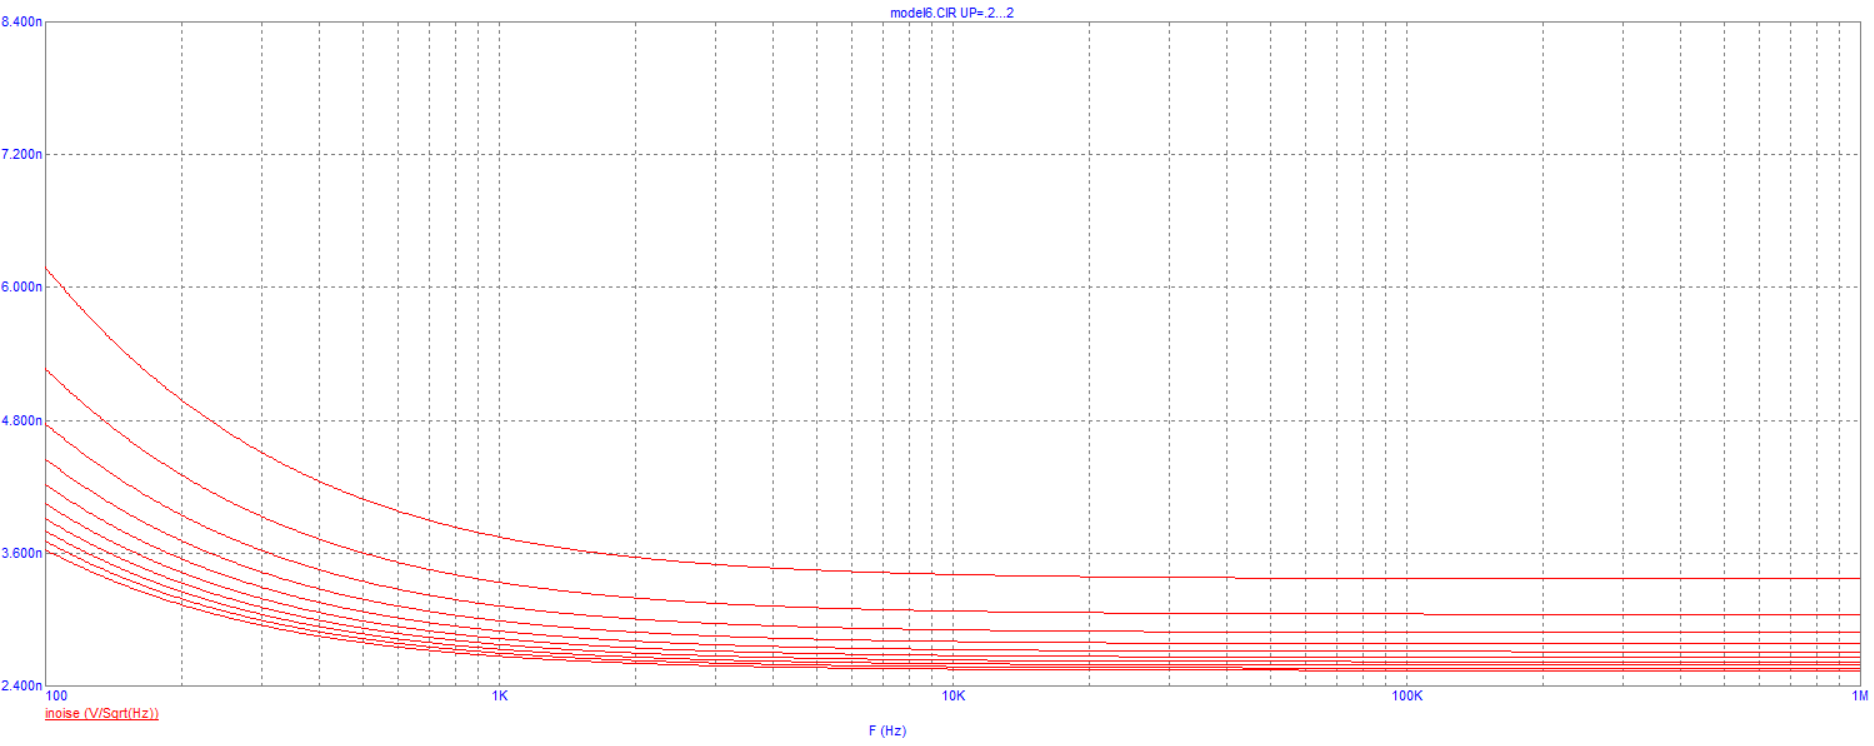
\includegraphics[scale=0.225]{images/mod6_1_2.png}
    \caption{Шумовой ток, варьирование $U_p$}
    \label{fig:m612}
\end{figure}

\begin{center}
\begin{table}[h!]
    \centering
    \begin{tabular}{|c|c|c|c|c|c|c|c|c|c|c|}
    \hline
        $U_p$ & 2.0 & 1.8 & 1.6 & 1.4 & 1.2 & 1.0 & 0.8 & 0.6 & 0.4 & 0.2\\ \hline
        $i_d$, p & 3.37 & 3.05 & 2.88 & 2.78 & 2.71 & 2.66 & 2.62 & 2.59 & 2.56 & 2.54 \\ \hline
    \end{tabular}
    \caption{Для $U_p = 1.1 V\, \gamma = \frac{i_d^2}{4kTS} \approx 0.65$}
    \label{tab:mt612}
\end{table}
\end{center}

\begin{figure}[h!]
    \centering
    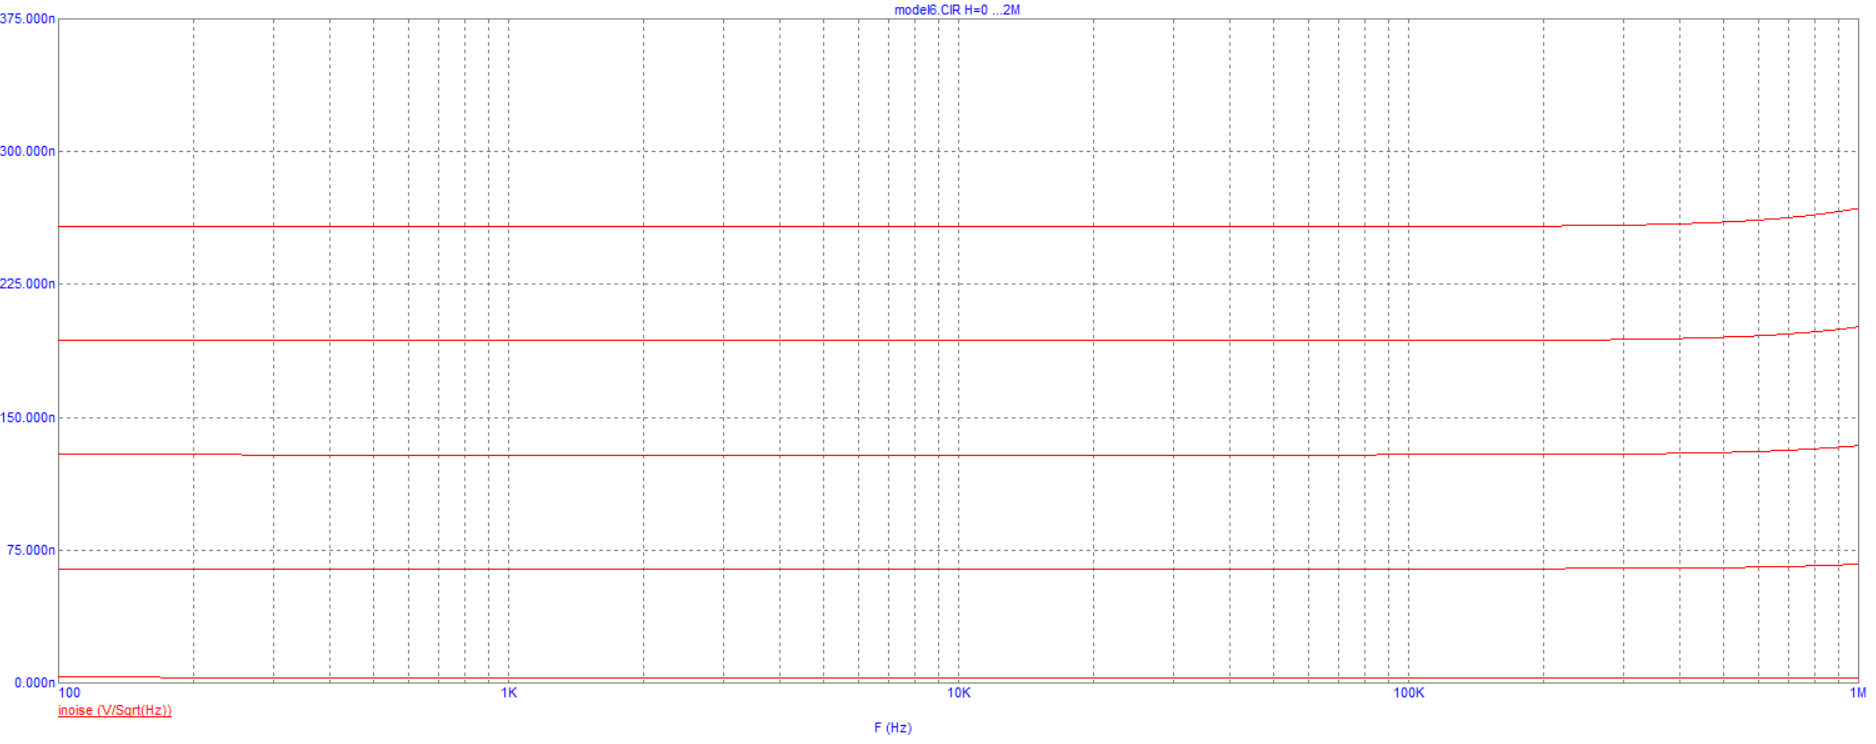
\includegraphics[scale=0.3]{images/mod6_1_3.png}
    \caption{Шумовой ток, варьирование Н}
    \label{fig:m613}
\end{figure}

\begin{center}
\begin{table}[h!]
    \centering
    \begin{tabular}{|c|c|c|c|c|c|}
    \hline
        $H$, Meg & 0 & 0.5 & 1 & 1.5 & 2\\ \hline
        $i_d$, n & 2.83 & 64.26 & 129.34 & 192.09 & 257.77 \\ \hline
    \end{tabular}
    \label{tab:mt613}
\end{table}
\end{center}

При мегаомном сопротивлении H ток совпадает с током при подключенном шумящем сопротивлении R, что неудивительно вследствии рассматриваемого диапазона частот и напряжений.

\subsection*{Исследование коэффициента шума}

\begin{figure}[h!]
    \centering
    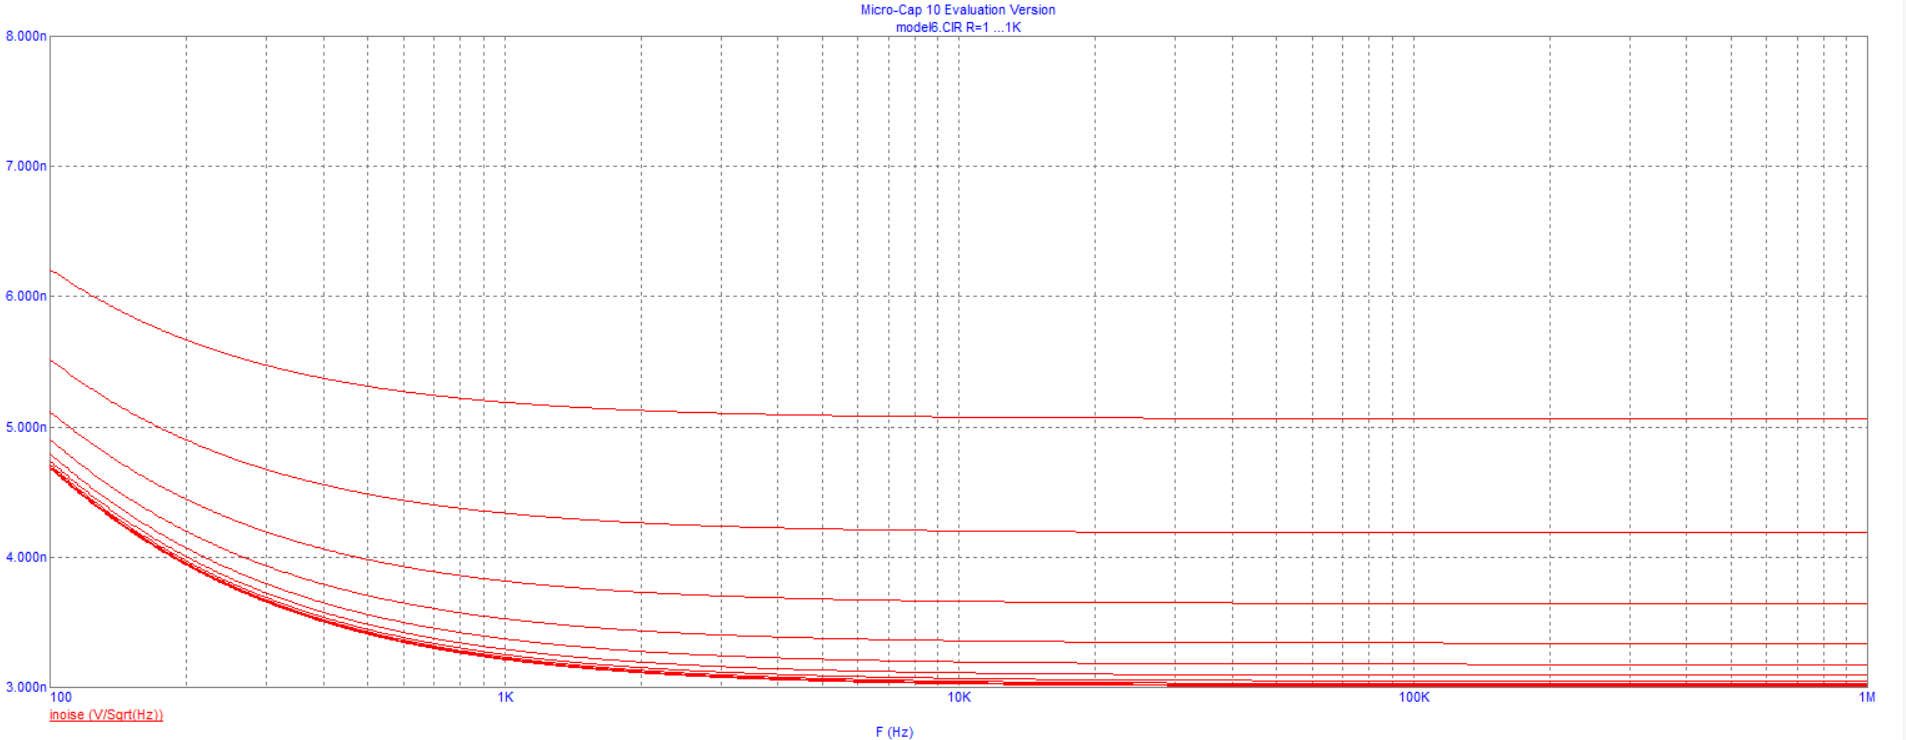
\includegraphics[scale=0.225]{images/2023-11-23_20-25-02.png}
    \caption{Шумовой ток, варьирование $R$}
    \label{fig:m612}
\end{figure}

Как видно, при сопротивлении R стремящемся к нулю, шумовое значение составит 3 нА. Шумовое сопротивление из формулы $R_n = \sqrt{\frac{\gamma R_g}{S}} \approx 18$ кОм. Шумовая температура составляет 300 К. А при $R = R_n$ шум на выходе равен $\sigma = 17.7$ нА.

\begin{figure}[h!]
    \centering
    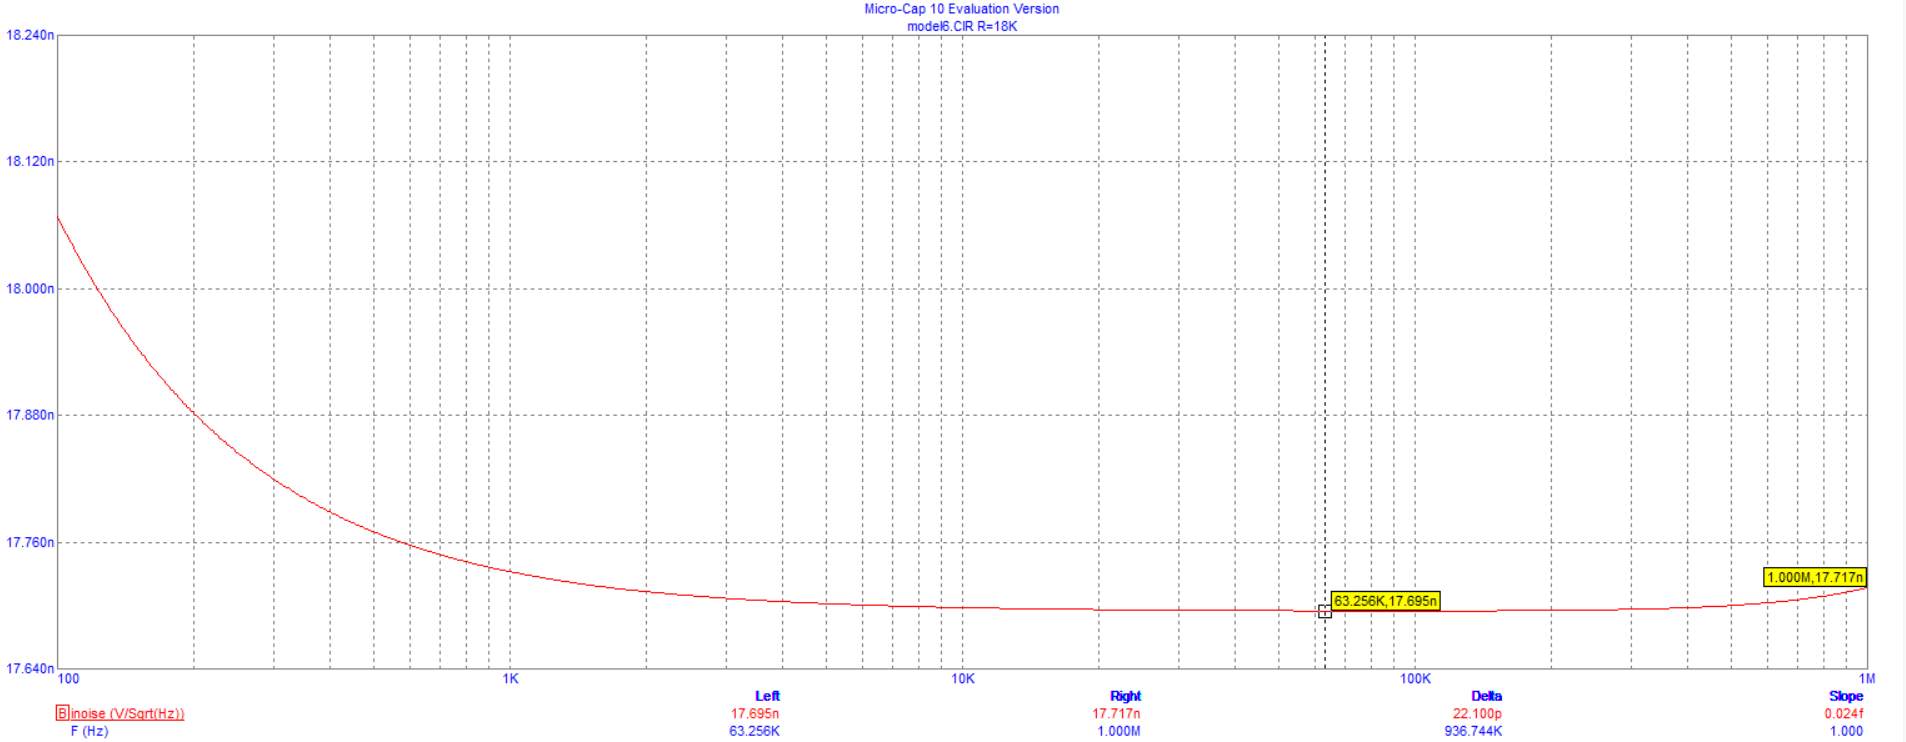
\includegraphics[scale=0.225]{images/2023-11-23_20-35-00.png}
    \caption{Шумовой ток, $R = R_n$}
    \label{fig:m612}
\end{figure}

\FloatBarrier

\end{enumerate}


\end{document}